\section{Semantic Web}
\label{cap2:semWeb}

\subsection{Web of Data}
\label{cap2:semWeb/webOfData}
During the short history of the World Wide Web, we have greatly benefited from how its 
content has been increasing every day while serving multiple purposes. This vast amount of 
knowledge has become humanly impossible to traverse, so we start relying on machines to 
process the content of documents automatically. As Hogan mentions, machines require the 
data to fulfill two primary requirements in order to be able to process them automatically 
in a meaningful way: to have a machine-readable structure and semantics~\cite{key:linked14-Hogan}. 
Unless a more \dquotes{formal} notion of structure and semantics is provided, machines can not 
be used to their full potential.

Various standards have emerged to partially structure the Web’s content, such as XML, CSV, 
or JSON. However, structured content without some semantics does not permit machines to do 
much more than split the content up by its delimiters and load its structure. Some other 
standards define semantic meaning for their structure, where some prominent examples are 
HTML, RSS or XML Schema (XSD), but often the semantics are defined in a human-readable way, 
for example, to describe how certain HTML elements should be rendered in a browser. Though 
these markup-based specifications provide a set of terms that often serve a singular purpose 
within the context of a given application, their interpretation tends to differ significantly 
for the respective consumer applications. 

The multiple purposes that standards like HTML can serve are not able to address some of the 
shortcomings of the current Web. Since content is often created to serve specific functionalities 
in the context of a given site, much of this content ends up not being directly reusable, 
high levels of redundancy appear or it cannot be integrated with other sites. In an effort 
to address these limitations, the Semantic Web was proposed.

The Semantic Web is designed as an extension of the current World Wide Web so as to enable 
the creation, sharing, and intelligent re-use of machine-readable content on the Web. The 
inception of the modern notion of the Semantic Web is founded on two major milestones: the 
original W3C recommendation of the first Resource Description Framework (\RDF{}) standard 
defining the core data model~\cite{key:oldrdf}, and the introduction of the vision for the 
Semantic Web outlined by Berners-Lee et al.~\cite{key:semwebsa}.

The vision of the Semantic Web can be represented through the Semantic Web Stack, first 
conceived by Berners-Lee et al., as seen in Figure~\ref{fig:semanticWebStack}. The lower levels describe the 
foundational elements of the Semantic Web which are aligned with the Web itself. First, 
the Web needs some standard to map from binary-streams and storage to textual information, 
so it relies on \textbf{Characters} from the standard Unicode character-set. Then, \textbf{Identifiers} 
respond to the main purposes of denoting any concept or concrete thing. The natural choice is to 
use Uniform Resource Identifiers (URI), which is the native standard for identification on 
the Web, or a recently adopted generalization of URI, Internationalized Resource 
Identifiers (IRI), which additionally support unescaped Unicode strings. The \textbf{Syntax} layer 
serves the objective of allowing machines to automatically parse content into its elementary 
components by defining syntaxes with formally defined grammars. For example, one of the most 
common syntaxes used to encode Semantic Web data is the Terse RDF Triple Language (Turtle) 
syntax~\cite{key:turtle}, based on the Notation3 (N3) syntax~\cite{key:n3}.

\begin{figure}[!h]
    \centering
    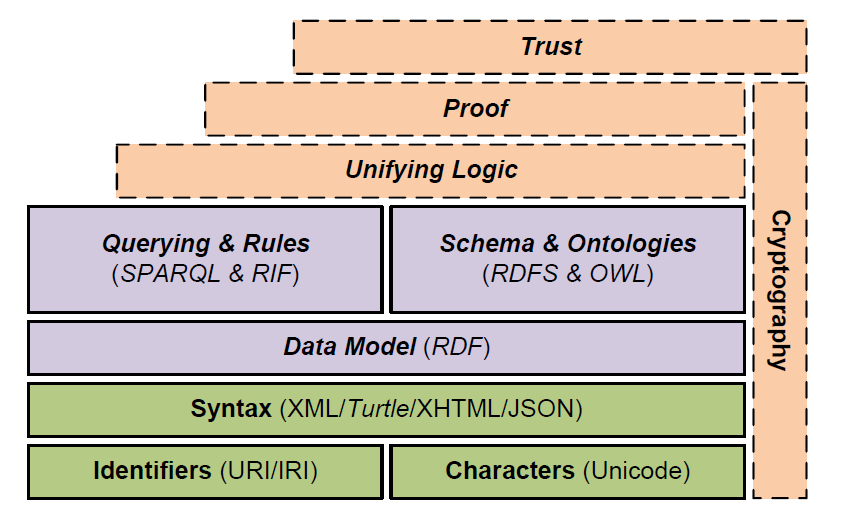
\includegraphics[scale=.65]{imagenes/2_theorical_framework/semanticWebStack.png}
    \caption{Semantic Web Stack~\cite{key:linked14-Hogan}}
    \label{fig:semanticWebStack}
\end{figure}

The next set of layers forms the core of the Semantic Web. The \textbf{Data Model} layer 
provides a canonical representation where machines can exchange machine-readable data in 
a generic framework. The core data-model for the Semantic Web is the Resource Description 
Framework (\RDF{})~\cite{key:rdfprimer}. In order to bring some meaning to the \RDF{} content, 
it requires formal languages whose meta-vocabulary complement the \RDF{} data-model by providing 
well-defined semantics. These languages correspond to the \textbf{Schema \& Ontologies} layer, 
where the RDF Schema (RDFS)~\cite{key:oldrdf} and Web Ontology Language (OWL)~\cite{key:owloverview, key:owl2rationale} 
standards are the essential languages integrated as part of the current Semantic Web. 
Eventually, the content described in \RDF{} needs to be processed by declarative querying 
and rules languages that serve many purposes, like generating results for user interfaces 
or inferring novel \RDF{} data. The \textbf{Querying \& Rules} layer is where the querying 
and rules standards for the Semantic Web are defined. In this case, the SPARQL Protocol 
and RDF Query Language~\cite{key:sparql,key:sparql11protocol,key:sparql11} 
defines the querying standards and the Rule Interchange Format (RIF)~\cite{key:rifframework} 
defines the rules standards.

The top and side of the stack in Figure~\ref{fig:semanticWebStack} are layers yet to be realized. Though many 
proposals have been made in the research literature, no mature standards or tooling have 
emerged. The remaining top layers aim to combine the described low-level technologies into 
a unifying language to execute queries and rules over knowledge represented in \RDF{} 
(Unifying Logic), provide proofs to validate procedures or information used (Proof), and 
determine the trustworthiness of information sources (Trust). The Cryptography side layer 
is centered on cryptographic techniques for verifying and allowing control access mechanisms.

Providing more details on this broad overview of the Semantic Web, we start by focusing on 
how data is represented and how querying the content is described by any selected source. 
Then, in the following sections, we go deeper into understanding the Semantic Web data-model, 
\RDF{}, and its querying standard, \SPARQL{}.

\subsection{Resource Description Framework}
\label{cap2:semWeb/rdf}
The \textbf{Resource Description Framework} (\RDF{}) standard~\cite{key:rdfprimer} provides 
a data-model on the Semantic Web, which can be serialized using the Turtle syntax~\cite{key:turtle}. 
Having this data-model allows for any content framed in \RDF{} to be generically processed 
and indexed by external systems, whatever its topic or origin. The atomic elements that 
constitute the \RDF{} data-model are called \textbf{\RDF{} Terms}. \RDF{} does not follow the Unique 
Name Assumption (UNA), so two \RDF{} terms can refer to the same referent. The set of \RDF{} terms 
are divided into three disjoint subsets: URIs, Literals and Blank Nodes.

As mentioned previously, \textbf{Uniform Resource Identifiers} serve as identification for 
any resource. An example to identify the country Chile in DBpedia~\cite{KG:dbpedia} is 
the URI \url{http://dbpedia.org/resource/Chile}. A shorter version can be used 
by using the CURIE-style shortcuts~\cite{key:prefixes}, where a re-usable prefix can be 
defined: \texttt{@prefix dbr: <\url{http://dbpedia.org/resource/}>}. This way, the 
identifier of Chile can be abbreviated to \texttt{dbr:Chile}.

% note: ^ is \textasciicircum, ~ is \textasciicircum, \ is \textbackslash
\textbf{Literal} values represent lexical values and are divided into two categories. 
Plain literals are a set of plain strings, such as \texttt{\dquotes{Hello World}}, and can 
include an associated language tag, such as \texttt{\dquotes{Hello World}@en}. Typed 
literals are literals that include a datatype, such as 
\texttt{\dquotes{8}\textasciicircum\textasciicircum xsd:int}. Datatypes are identified by 
URIs (such as \texttt{xsd:int}) and borrow most of the datatypes defined for XML 
Schema~\cite{key:xsd}. Datatypes are often used for data validation or mapping.

\textbf{Blank Nodes} are used as existential variables that denote the existence of some 
resource without having to explicitly reference it using a URI or literal. The scope of a 
blank node is limited to the local \RDF{} document where it is defined, so it cannot be 
referenced elsewhere. In Turtle, blank nodes can be referenced explicitly with an 
underscore prefix \texttt{\_:bnode1} or implicitly in a variety of other manners.

\RDF{} terms are then combined together to form \RDF{} Triples. As its name suggests, a triple 
is a 3-tuple of \RDF{} terms. The three components of a triple are commonly called subject, 
predicate and object. \RDF{} triples can be seen as an atomic representation of a 
\dquotes{fact} or \dquotes{claim}, e.g. \dquotesit{Santiago is the capital city of Chile}. 
Typically each \RDF{} triple position fulfills a certain role: the subject is the primary 
resource that is being described (either a URI or a blank node), the predicate is the 
relation between the subject and the object (must be a URI), and the object is the value 
of the relation (any of the mentioned \RDF{} terms). For instance, we illustrate the Turtle 
representation of a set of \RDF{} triples from DBpedia in Listing~\ref{lst:dbpediaRdfExample}.

\begin{sparqlcode}[caption={Set of \RDF{} triples about Gabriela Mistral in DBpedia using Turtle syntax.},label={lst:dbpediaRdfExample}]
# PREFIX DECLARATIONS
@prefix dbr: <http://dbpedia.org/resource/>
@prefix dbo: <http://dbpedia.org/resource/>
@prefix dbp: <http://dbpedia.org/resource/>
@prefix rdfs: <http://www.w3.org/2000/01/rdf-schema#>

# RDF TRIPLES
dbr:Gabriela_Mistral rdfs:label "Gabriela Mistral"@en .
dbr:Gabriela_Mistral dbp:occupation dbr:Poet .
dbr:Gabriela_Mistral dbo:birthPlace dbr:Vicuña,_Chile .
dbr:Gabriela_Mistral dbo:awards dbr:Nobel_Prize_in_Literature .
dbr:Gabriela_Mistral dbo:awards dbr:National_Prize_for_Literature_(Chile) .
dbr:Vicuña,_Chile rdfs:label "Vicuna, Chile"@en .
dbr:Vicuña,_Chile dbo:populationTotal 25085 .
dbr:Vicuña,_Chile dbo:isPartOf dbr:Elqui_Province .
dbr:Vicuña,_Chile dbo:isPartOf dbr:Coquimbo .
dbr:Vicuña,_Chile dbo:country dbr:Chile .
\end{sparqlcode}

Listing~\ref{lst:dbpediaRdfExample} shows facts about Gabriela Mistral, a famous Chilean poet, 
and how those facts are structured as a set of \RDF{} triples, where each triple is separated by a 
dot symbol. The use of CURIE-style prefixes helps to simplify the content and make it easier to 
understand for a human reader~\cite{key:prefixes}. Moreover, Listing~\ref{lst:dbpediaShortRdf} 
shows how Turtle allows for abbreviating the content by grouping triples with common subjects 
(using the \squotestt{;} symbol) or predicates (using the \squotestt{,} symbol).

\begin{sparqlcode}[label={lst:dbpediaShortRdf},caption={Set of \RDF{} abbreviated triples about Gabriela Mistral in DBpedia.}]
...
# RDF TRIPLES
dbr:Gabriela_Mistral rdfs:label "Gabriela Mistral"@en ;
    dbp:occupation dbr:Poet ;
    dbo:birthPlace dbr:Vicuña,_Chile ;
    dbo:awards dbr:Nobel_Prize_in_Literature, dbr:National_Prize_for_Literature_(Chile) .
dbr:Vicuña,_Chile rdfs:label "Vicuña, Chile"@en ;
    dbo:populationTotal 25085 ;
    dbo:isPartOf dbr:Elqui_Province , dbr:Coquimbo ;
    dbo:country dbr:Chile .
\end{sparqlcode}

Given the triple-based structure of \RDF{} triples, it is possible to represent entire 
datasets as an \RDF{} graph, also known as a \textbf{Knowledge Graph}: a directed labeled 
graph where subjects and objects are represented by nodes, and predicates are represented 
by the directed edges that bond two nodes. The \RDF{} graph of the example shown above can be 
drawn as in the diagram of Figure~\ref{fig:dbpediaGraphExample}, where by convention 
ellipses correspond to URIs or blank nodes, and rectangles symbolize literals.

\begin{figure}[!h]
    \centering
    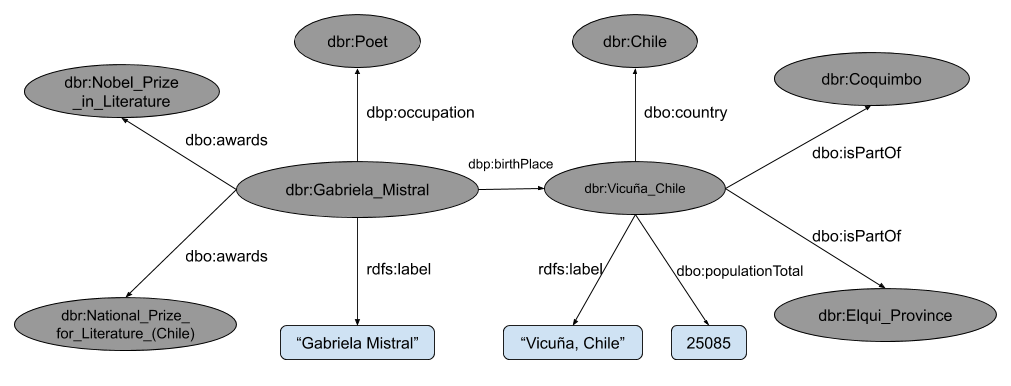
\includegraphics[scale=.55]{imagenes/2_theorical_framework/exampleDbpediaGraph.png}
    \caption{\RDF{} graph representing facts about Gabriela Mistral from Listing~\ref{lst:dbpediaRdfExample}.}
    \label{fig:dbpediaGraphExample}
\end{figure}

Besides \RDF{} triples and \RDF{} graphs, \RDF{} standards provide a rich set of built-in 
vocabulary terms under a core \RDF{} namespace, which helps to standardize frequently used 
\RDF{} patterns. One popular term is \texttt{rdf:type}, which helps to assign resources 
sharing certain commonalities into \textbf{classes}. For example, we can denote 
\texttt{dbr:Vicuna\_Chile} as a city by combining it with the predicate \texttt{rdf:type} 
and the object \texttt{dbr:City}. Another example is the term \texttt{rdfs:label} that 
comes from RDF Schema~\cite{key:rdfsold}. which provides other resources for describing 
relations such as \textbf{subproperties} or \textbf{subclasses}. Though our work is not 
focused on the use of the Web Ontology Language (OWL)~\cite{key:owl2rationale, key:owloverview}, 
it is worth mentioning that it also adds a wealth of new vocabulary to describe new 
relations between resources like equivalences, disjointness, inverse properties, among others.

Ultimately, there are numerous syntaxes for writing \RDF{} apart from Turtle~\cite{key:turtle}, among 
which we can name RDF/XML~\cite{key:rdfxml}, N-Triples~\cite{key:testcases}, RDFa~\cite{key:rdfa11p, key:rdfa}, 
and JSON LD~\cite{key:jsonld}. However, no matter what syntax is chosen, every one is 
represented in the same \RDF{} data model; thus it is possible to convert any \RDF{} content 
in one syntax to another while keeping the same \RDF{} data.

\subsection{SPARQL Query Language}
\label{cap2:semWeb/sparql}
The \textbf{SPARQL} protocol defines how \SPARQL{} queries retrieve results over the \RDF{} 
data-model~\cite{key:sparql11protocol}. These standards became W3C Recommendations in 
2008~\cite{key:sparql} and then were extended in 2013 in the SPARQL 1.1 version~\cite{key:sparql11} 
superseding the previous W3C Recommendations. Some \SPARQL{} query features and keywords are similar 
to the ones found in the Structured Query Language (SQL), though \SPARQL{} is designed for interacting 
with \RDF{} data.

\begin{sparqlcode}[%
    caption={\SPARQL{} query for getting awards won by people who were born in Vicuña.},
    label={lst:dbpediaSparqlExample}]
# PREFIX DECLARATIONS
PREFIX dbr: <http://dbpedia.org/resource/>
PREFIX dbo: <http://dbpedia.org/ontology/>
# DATASET CLAUSE
FROM <http://dbepdia.org/data/Gabriela_Mistral.ttl>
# RESULT CLAUSE
SELECT ?people ?award
# QUERY CLAUSE
WHERE {
    ?people dbo:birthPlace dbr:Vicuña,_Chile,
        dbo:award ?award .
}
# SOLUTION MODIFIERS
LIMIT 2
\end{sparqlcode}

There are five main components that describe a \SPARQL{} query. First, \textbf{Prefix Declarations} 
serve as shortcuts for later in the query, similar to the Turtle shortcuts. Following prefixes, 
the \textbf{Dataset Clause} allows for specifying one or more \RDF{} graphs over which the query 
should be executed. When no dataset clause is specified, query patterns are matched against the 
default graph which usually corresponds to all of the data loaded and indexed. The 
\textbf{Result Clause} indicates what type of query is being executed and what results are expected. 
The most relevant part is the \textbf{Query Clause}, where the query patterns to match against the 
data are specified and used to generate variable bindings. Finally, the \textbf{Solution Modifiers} 
permit to order, slice or paginate the results. Note that the only mandatory part is the result 
clause, though most queries also include at least one query clause. An example of a \SPARQL{} query is 
represented in Listing~\ref{lst:dbpediaSparqlExample}, where we are looking for which awards 
people who were born in Vicuña have won.

For example, if the \RDF{} triples shown in Listing~\ref{lst:dbpediaRdfExample} were contained in the 
\RDF{} graph \texttt{<\url{http://dbpedia.org/data/Gabriela\_Mistral.ttl}>}, the results 
expected from the \SPARQL{} query in Listing~\ref{lst:dbpediaSparqlExample} would be as shown 
in Table~\ref{table:dbpediaExampleResults}.

\begin{table}[h!]
    \centering
    \begin{tabular}{ |c|c| }        
        \hline
        ?people & ?award \\ 
        \hline
        dbr:Gabriela\_Mistral & dbr:Nobel\_Prize\_in\_Literature \\
        dbr:Gabriela\_Mistral & dbr:National\_Prize\_for\_Literature\_(Chile) \\
        \hline
    \end{tabular}
    \caption{Results from \SPARQL{} query example in Listing~\ref{lst:dbpediaSparqlExample}.}
    \label{table:dbpediaExampleResults}
\end{table}

There are four types of \SPARQL{} queries, which are defined by the first keyword used in the 
\textit{Result Clause}. The example shown above is a \texttt{SELECT} query, which requests a list 
of bindings for variables specified in the \textit{Query Clause}. Since a \texttt{SELECT} query 
returns duplicate results by default, it can include either the \texttt{DISTINCT} keyword to filter 
duplicate results, or the \texttt{REDUCED} keyword that may allow duplicates such that the engine 
can choose whatever it deems to be more efficient. An \texttt{ASK} query returns a boolean value 
indicating whether or not the query’s results are non-empty. A \texttt{CONSTRUCT} query provides 
an \RDF{} template with placeholders to be filled later, thus returning an \RDF{} graph according to 
those inserted variables. The last type is the \texttt{DESCRIBE} query, which provides an \RDF{} 
description for a particular \RDF{} term. For this work we only focus on \texttt{SELECT} and 
\texttt{ASK} queries.

Knowing how to define the content inside a \textit{Query Clause} is crucial to specify what results 
a \SPARQL{} query should return. There are many core features defined over the basic graph patterns 
that are used to create complex query patterns in query clauses. Among these patterns, we highlight 
the \texttt{FILTER} keyword that serves to establish conditions that a query solution should match. 
These conditions can be constructed from a broad arsenal of tools: arithmetic operators and 
comparators, built-in functions, casting, boolean connectives and even user-defined functions. 
We also mention the \texttt{UNION} operator, that allows joining results from two groups of query 
patterns. Another important feature is the \texttt{OPTIONAL} feature, which allows for matching 
data if available (if not, the corresponding result is still returned, where the variables 
exclusive to the \texttt{OPTIONAL} clause are left unbound).

After retrieving results from the \textit{Query Clause}, such results can be divided or modified. 
The \texttt{ORDER BY} operation sorts results in ascending (ASC) or descending (DESC) order based 
on one or more variables; and the \texttt{LIMIT} keyword restricts the amount of results to return. 
Finally, the \texttt{OFFSET} clause allows the query to skip a certain number of results.

Besides the basic operations provided by the original \SPARQL{} standard, the later update to 
SPARQL 1.1~\cite{key:sparql11} brought a wide-range of new features that increase the expressiveness 
and capabilities of this query language. Some core additions are property paths, aggregation, 
binding variables, subqueries, updates, new format outputs (CSV, TSV, JSON), among others. 
For this work we want to highlight the use of \textit{property paths} and \textit{aggregation}, 
that will be often used. \textit{Property paths} allow the user to match paths of arbitrary 
length in an \RDF{} graph using regular expressions. \textit{Aggregation} techniques include 
operations like count, max, min, sum, etc.; and can be applied over query results grouped 
by common terms.

Though many other \SPARQL{} features are left to be mentioned, we focused on the features described 
above since those are the important ones for the development of this work.

\subsection{Linked Open Data Cloud}
\label{cap2:semWeb/linkedData}
Having briefly mentioned some core components of the Semantic Web, we have scratched just a tiny 
portion of what the Semantic Web concept means, and how it can be deployed on the Web. Most of 
what defines the use of the Semantic Web on the Web itself resides in understanding 
\textbf{Linked Data}. The early attempts to publish \RDF{} on the Web tended to produce large dumps 
of data rarely interlinked with other \RDF{} datasets and using different conventions. These issues 
ended up leaving entire isolated islands of \RDF{} datasets that were difficult to access and with 
little chance of being discovered by other communities. Therefore, \textit{Linked Data} emerged as 
a set of principles and best practices~\cite{key:ldprinciples} to provide an environment where 
Semantic Web standards can be effectively deployed on the Web.

The four Linked Data principles arise from the Web Design Issues document published by 
Berners-Lee\cite{key:ldprinciples}. According to this document, these principles are: (1) use URIs 
as names for things, (2) use HTTP URIs so those names can be looked up, (3) return useful 
information upon lookup of those names, and last (4) include links by using URIs that dereference 
to remote documents. 

Besides these principles, there is an emphasis on publishing data that can be easily processed, 
reused and exchanged between machines. As an approach to bootstrap Semantic Web publishing, 
a 5-star system\cite{key:ldprinciples} was promoted to describe the quality of published \RDF{} data. 
Each star corresponds to one of the following considerations: (1) publish data under an open license, 
(2) publish structured data, (3) use non-proprietary formats, (4) use URIs to identify things, and 
(5) link the published data to other data.

A community project named \dquotesit{Linking Open Data}, supported by W3C and inspired by the growth 
in Open Data, emerged to promote these Linked Data principles~\cite{key:ldbook}. The community 
project aims to introduce the benefits of Semantic Web technologies to the Open Data movement and 
to bootstrap the Web of Data by including many emerging open datasets. The community published 
guidelines are based on the core principles mentioned before. Among those guidelines, the main 
ones are:

\begin{itemize}
    \item \textbf{Dereferencing practices}: sets a guide on how to identify and perform lookups 
    for either entities or documents. This includes recommendations on indirect URIs to signify 
    distinctions on a HTTP level or providing as detailed an \RDF{} description as possible when 
    dereferencing resources. 
    \item \textbf{Linking Aliases}: allow the use of multiple URI aliases that refer to the same 
    thing. For example, \textit{owl:sameAs} links can be used to specify equivalence between 
    resources in different datasets.
    \item \textbf{Describing Vocabularies Terms}: promotes the shared use of common vocabularies 
    of class and property terms. A common example is to use FOAF to describe people [ref].
    \item \textbf{Provision of SPARQL Endpoints}: though not required, providing a \SPARQL{} endpoint 
    for a given Linked Data site gives consumers a single-point-of-access to query over the merge 
    of contributions on that site.
\end{itemize} % TODO: check why itemize put so much space between items (removing following section line reduces the space to normal)

Based on these standards and guidelines, the \textbf{Linking Open Data Cloud}, a set of more than 
300 different interlinked \RDF{} datasets, has been constantly growing and including a wider range of 
topics. Some of the most relevant datasets are DBpedia~\cite{KG:dbpedia}, whose content is mostly 
based on Wikipedia articles, Freebase~\cite{KG:freebase}, a dataset previously supported by Google, 
and Wikidata~\cite{KG:wikidata}, a large dataset supported by its community. Our work is mainly 
focused on the latter knowledge graph, which we will introduce in the next section.

\subsection{Wikidata}
\label{cap2:semWeb/wikidata}
As described by Vrandečić and Krötzsch~\cite{KG:wikidata}, \textbf{Wikidata} is a free 
collaborative knowledge graph founded by the Wikimedia Foundation\footnote{\url{https://wikimediafoundation.org/our-work/wikimedia-projects/}} 
in October 2012. Given the constant growth of its sister project Wikipedia, one of the most 
popular online encyclopedias, Wikidata is introduced as a new multilingual 
\dquotesit{Wikipedia for data}. 

Despite Wikipedia’s rich amount of data, consisting of more than 30 million articles in at least 
287 languages, it started to face serious limitations in terms of providing data easily to the 
community~\cite{KG:wikidata}. There was the lack of direct access through query services or 
downloadable data exports, the same information often needed to be manually maintained in the 
same articles across many languages and across many articles within a single language, among 
others limitations. Wikidata aims to overcome many of Wikipedia’s limitations by managing its 
data centrally.

Wikidata offers many features that make it an attractive and potentially useful resource for 
sharing information and connecting communities. Some aspects to consider about Wikidata are:

\begin{itemize}
    \item \textbf{Openly editable}: allows any user to extend and edit the stored information.
    \item \textbf{Community control}: contributor community control that not only supervises the 
    data being published but also the schema of the data. 
    \item \textbf{Plurality}: though many facts can be disputed or be uncertain, Wikidata provides 
    mechanisms to organize conflicting data for coexisting together.
    \item \textbf{Secondary data}: gathers facts published in primary sources including references 
    to these sources.
    \item \textbf{Multilingual data}: all data have universal meaning and most of it is not tied 
    to a single language. There is only one universal version of Wikidata.
    \item \textbf{Easy access}: data published under liberal legal terms are made  easily 
    accessible through web services, allowing the widest possible reuse.
    \item \textbf{Continuous evolution}: Wikidata grows with its community of editors and 
    developers, so new features are constantly being added.
\end{itemize}

Wikidata has its own data model but further offers exports that follow the Semantic Web 
standards~\cite{key:wikidataErxlebenGKMV14}. To identify items, Wikidata provides unique IDs, 
which are highly reusable and provide unambiguous definitions that do not depend on language 
labels. The same example of the entity Chile mentioned before is now represented in Wikidata as 
\texttt{\url{http://www.wikidata.org/wiki/Q298}}. 

\begin{sparqlcode}[%
    caption=Set of RDF triples about Gabriela Mistral in Wikidata., 
    label=lst:wikidataRdfExample]
# PREFIX DECLARATIONS
@prefix wd: <http://wikidata.org/wiki/>
@prefix wdt: <http://wikidata.org/prop/direct/>
@prefix p: <http://wikidata.org/prop/>
@prefix pq: <http://wikidata.org/prop/qualifier/>
@prefix rdfs: <http://www.w3.org/2000/01/rdf-schema#>

# RDF TRIPLES
# Gabriela Mistral
wd:Q80871 rdfs:label "Gabriela Mistral"@en ;
    wdt:P106 wd:Q49757 ;
    wdt:P19 wd:Q201007 ;
    wdt:P166 wd:Q37922, wd:Q860699 .
# Vicuna
wd:Q201007 rdfs:label "Vicuña"@en ;
    p:P1082 _:population2017 ;
    wdt:P131 wd:Q721224 ;
    wdt:P17 dbr:Chile .
_:population2017 pq:P1082 25085
# Elqui Province
wd:Q721224 wdt:P131 wd:Q2121 .
\end{sparqlcode}

Since some facts can not be directly expressed by simply using the property-value convention, 
like the population of Chile across different years, Wikidata also provides additional 
subordinate property-value pairs called \dquotesit{qualifiers}. \textbf{Qualifiers} can be used 
to state contextual information such as validity time or ternary relations (e.g. cast members of 
a movie with their role). Another way to understand qualifiers is by looking at Wikipedia 
infoboxes which have a similar data representation.

\begin{figure}[!h]
    \centering
    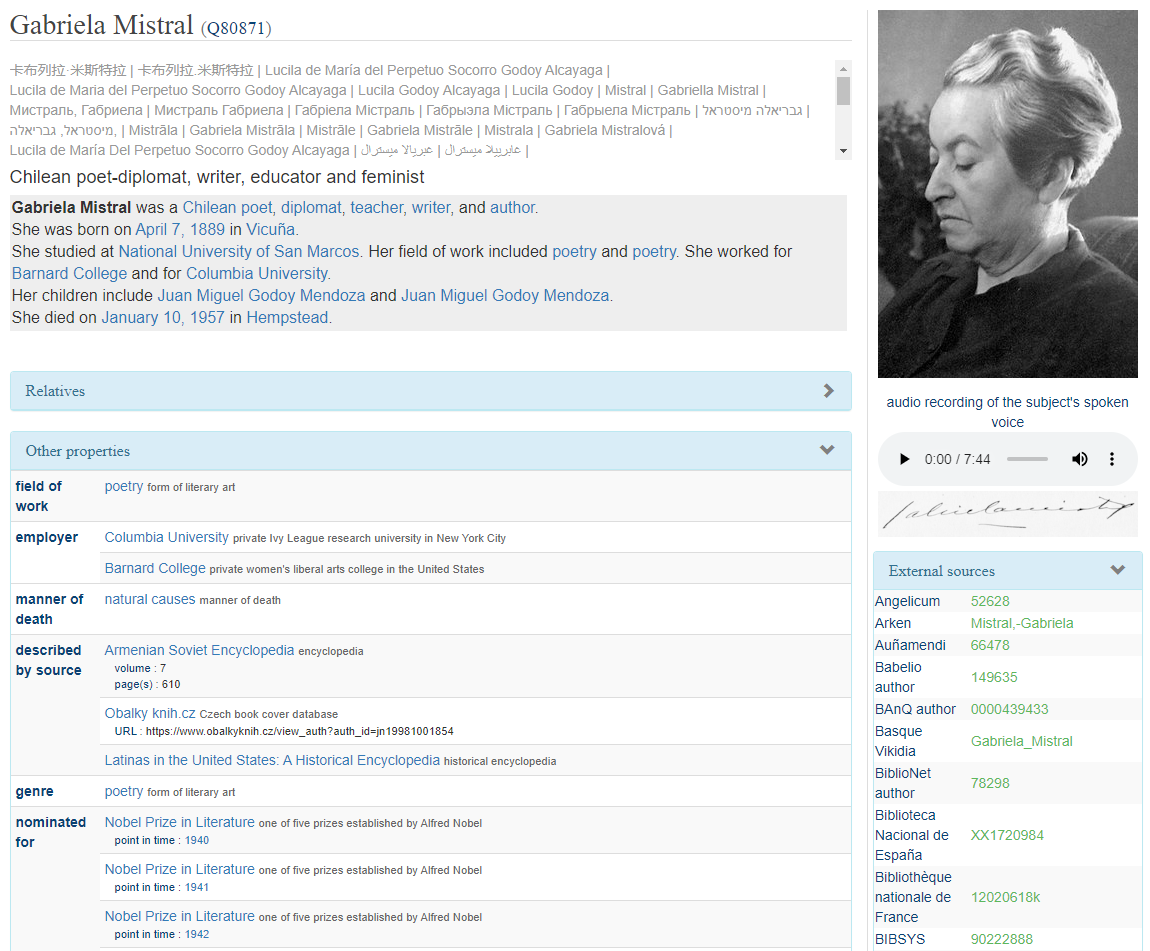
\includegraphics[scale=.5]{imagenes/2_theorical_framework/wikidataReasonatorExample.PNG}
    \caption{Example of an external application of Wikidata using Reasonator.}
    \label{fig:wikidataReasonator}
\end{figure}

For a better understanding, let us recall the same data about Gabriela Mistral, but now using 
Wikidata resources, as shown in Listing~\ref{lst:wikidataRdfExample}. Since different knowledge 
graphs do not necessarily represent the same information in the same way, we can appreciate slight 
differences like how the city Vicuña is described. In this case, Vicuña is not directly represented 
as part of Coquimbo but instead only Elqui Province. Nevertheless, both representations are 
intrinsically correct since both are portraying the same fact. Another difference is the use of 
a Wikidata property qualifier to denote that the population for Vicuña shown in 
Listing~\ref{lst:wikidataRdfExample} is the population of 2017, in contrast to the DBpedia 
representation, shown in Listing~\ref{lst:dbpediaShortRdf}, which does not show that fact.

Ultimately, the data in Wikidata lends itself to numerous applications on very different levels 
of data integration. Wikidata provides many language labels and descriptions for many terms in 
different languages, which allows any service to present and/or or translate information for 
various audiences. Some applications are built to access Wikidata’s data more conveniently and 
effectively. One example is illustrated by Figure~\ref{fig:wikidataReasonator}, showing 
information about Gabriela Mistral retrieved by the data browser 
Reasonator\footnote{\url{https://reasonator.toolforge.org/}} using the Wikidata API. Additionally 
applications can be enriched with information provided by Wikidata, such as how Google Maps 
uses Wikidata’s geographical labels to enhance its application interface. 

On a more advanced level, many research analyses can be performed over the information in 
Wikidata in order to derive new insights beyond its surface data. A couple of potential examples 
are analyses using logical reasoning to understand intrinsic meaningful relationships among 
entities, or statistical evaluations over the data to analyze biases like the ones that involve 
language coverage~\cite{key:wikidataHale13} or gender balance~\cite{key:socialWikidataWagner16}. 
Wikidata is already an important platform and has the potential to be a major resource for both 
researchers and developers~\cite{wikidata:GeneWikiInitiative, wikidata:RiseWikidataVrandecic6682924}.
